% DSA4212 - Optimisation for Large-Scale Data-Driven Inference
% Small-LLM project, final report. Course Overleaf template (12pt, natbib, libertine).
% Compile from report/: pdflatex final_report; bibtex final_report; pdflatex twice.
% Figures: report/figures/. Bibliography: report/final_references.bib.
\documentclass[12pt]{article}
\usepackage[T1]{fontenc}

%%%%%%%%%%%%%%%%%%%%%%%%%%%%%%%%%%%%%%%%%%%%%%%%%%%%%%%%%%%%%%%%%%%%%%%%%%%%%%%%%%%%%%
%%%%%%%%%%%%%%%%%%% YOU PROBABLY DON"T NEED TO CHANGE ANYTHING HERE %%%%%%%%%%%%%%%%%%%
\usepackage[numbers,sort]{natbib}
\usepackage{amsfonts, amsmath}
\usepackage{graphicx}
\usepackage{booktabs}
\IfFileExists{libertine.sty}{\usepackage{libertine}}{\IfFileExists{lmodern.sty}{\usepackage{lmodern}}{}}
\usepackage{fullpage}
\usepackage{hyperref}
\hypersetup{
    colorlinks = true,
    linkcolor = blue,
    urlcolor  = blue,
    citecolor = blue,
    anchorcolor = blue}
\urlstyle{same}
\IfFileExists{microtype.sty}{\usepackage{microtype}}{}
\setlength{\emergencystretch}{3em}
\Urlmuskip=0mu plus 1mu\relax
%%%%%%%%%%%%%%%%%%%%%%%%%%%%%%%%%%%%%%%%%%%%%%%%%%%%%%%%%%%%%%%%%%%%%%%%%%%%%%%%%%%%%%
\usepackage[font=small]{caption}
\setlength{\textfloatsep}{10pt plus 2pt minus 2pt}
\setlength{\bibsep}{2pt}
\renewcommand{\topfraction}{0.9}\renewcommand{\bottomfraction}{0.8}
\renewcommand{\textfraction}{0.05}\renewcommand{\floatpagefraction}{0.85}

\author{}
\title{Training a small GPT on TinyStories in one hour:\\
model size against the tokens it can see}
\date{November 2026}

\begin{document}
\maketitle
\vspace{-4em}

{\bf Group Composition:}
\begin{enumerate}\setlength{\itemsep}{0pt}
\item Kerem Ozemre, A0350378Y
\item Tonio Kowalke, A0350429E
\item Steffany Lara, A0350565H
\item Ahmed Haj Hassine, A0342398U
\end{enumerate}

{\bf Github Repository:}
\href{https://github.com/KeremOzemre/Optimization-for-Large-Scale-Data}{github.com/KeremOzemre/\allowbreak Optimization-for-Large-Scale-Data}

\begin{abstract}
\noindent GPT models are trained from random weights on TinyStories, each run for one hour
on the same GPU slice. A first comparison spans five model sizes (16M to 253M
parameters) and four fractions of the training data, 20 runs in total. The 124M
model (XL) has the lowest loss. The 253M model (XXL) is not better, although it has
twice the parameters, because in one hour it processes only half as many tokens.
The first comparison had one seed and unequal validation samples, so it was checked
twice: the saved checkpoints were scored again on the complete validation set, and
XL and XXL were trained again with three seeds each. XL wins in all three pairs
(mean cross-entropy 1.4947 against 1.5244, about 2.9\% lower perplexity). The amount
of training data changes the loss by about 0.01 nats or less. The
validation-selected model reaches a test perplexity of 4.41 (0.524 bits per byte).
A matched-token control settles why XXL loses: trained on the same 143M tokens with
a step-based schedule, XXL beats XL by 0.053 nats, so XXL runs out of clock, not of
capacity. Halving XXL's learning rate did not close the one-hour gap.
\end{abstract}

\section{Budget, initialisation and evaluation objective}
\label{sec:budget}
\textbf{Budget.} The budget was fixed before the final runs: 3600 seconds of
wall-clock time inside the training loop for each run, on one NVIDIA H100 NVL MIG
slice (\texttt{3g.47gb}), in \texttt{bfloat16}. The timer includes the periodic
validation and logging. Data preparation, model creation, the final validation and
saving the checkpoint are outside the timer. No run was resumed. The 20 runs of the
first comparison and the 6 repeated runs use 26 slice-hours of one-hour training.
The matched-token pair (Section~\ref{sec:xlxxl}) uses a step budget of 35{,}000
updates instead of the clock and, with the reduced-rate one-hour run, adds about
2.5 slice-hours on the same MIG slice. Four extra runs (Section~\ref{sec:extensions})
add 2.5 hours on a GPU with a different label, and are treated separately. Pilot
runs and all offline scoring are not in the budget.

\textbf{Initialisation.} All models start from random weights with the nanoGPT
initialisation~\cite{nanogpt}. No pretrained weights or embeddings are used. The
only external component is the GPT-2 tokenizer, which the project rules allow.

\textbf{Evaluation objective.} The metric is cross-entropy (CE, nats per token) on
held-out TinyStories text. It is the quantity the model is trained on, so it reads
language-modelling quality directly. Perplexity, $\exp(\text{CE})$, and bits per
byte are also reported for the test set, because per-token numbers cannot be
compared with groups that use another tokenizer. These metrics say how well the
model predicts the next token. They do not say if a generated story is coherent, so
samples are also read (Section~\ref{sec:test}), without scoring them.

\section{Research question and background}
The question is practical: \emph{with one hour on a fixed GPU, which model size
predicts held-out text best, and does it matter how much training data is
available?}

A larger model can fit more patterns, but every update costs more. With a fixed
clock, more capacity means fewer updates and fewer tokens seen. Kaplan et
al.~\cite{kaplan2020} find that large models are more sample-efficient, and that
with a fixed amount of compute the best choice is a large model that stops well
before convergence. Hoffmann et al.~\cite{hoffmann2022} correct the balance: model
size and training tokens should grow together, at about 20 tokens per parameter.
Both results are for much larger models and data, and their budget is FLOPs, not
time. Two sources are closer to this setting. Geiping and
Goldstein~\cite{geiping2023} train a language model for one day on one GPU and
report that the loss per gradient step falls faster for models with more
parameters, but those models are slower, so the two effects almost cancel out.
An informal experiment with five minutes on a laptop~\cite{goedecke}, also on
TinyStories, finds the best size near 2M parameters, close to the 20 tokens per
parameter rule. So the literature gives two predictions for one hour that do not
agree: ``as large as possible, stop early''~\cite{kaplan2020} or ``about one
parameter for every 20 tokens''~\cite{hoffmann2022}. This report measures which one
is closer.

For the data axis, the reference is Muennighoff et al.~\cite{muennighoff2023}:
they report that repeating data for up to about four epochs costs almost nothing.
The small models here repeat the 25\% subset about eight times, a bit beyond that
range.

TinyStories~\cite{tinystories2023} was chosen because it was built for small
models: models with a few million parameters already write simple, mostly correct
stories. Differences between the configurations should then be visible in one hour.

\section{Experimental setup}
\textbf{Data.} \texttt{roneneldan/TinyStories} from Hugging Face. The training
split has 2,119,719 stories (473,992,236 tokens). The official validation set is
split 80/20 at story level with seed 42, which gives 17,592 validation stories
(3,808,644 tokens) and 4,398 test stories (957,274 tokens). The 25/50/75\% subsets
have about 118, 237 and 355 million tokens. The dataset was not checked for
duplicated stories.

\textbf{Tokenizer.} GPT-2 BPE from \texttt{tiktoken} (50,257 entries), with an
end-of-text token after each story. It is the same for all runs.

\textbf{Model.} The nanoGPT decoder-only Transformer~\cite{nanogpt,vaswani2017}:
causal attention, learned position embeddings, tied input and output embeddings,
context length 256, dropout 0.1. Table~\ref{tab:sizes} lists the five sizes. Depth,
width and number of heads change together, so their effects cannot be separated.

\begin{table}[htbp]
  \centering\small
  \caption{The five model sizes. The effective batch is always 16 sequences (4096
  tokens) per update. The last three columns are for the 100\% data runs of the
  first comparison.}
  \label{tab:sizes}
  \begin{tabular}{lrrrrrrr}
    \toprule
    Size & Layers & Width & Heads & Params (M) & Micro $\times$ accum. & Tokens/s (k) & Tokens (M) \\
    \midrule
    Small  &  4 &  256 &  4 &  16.08 & $16 \times 1$ & 273.4 & 984.3 \\
    Medium &  6 &  384 &  6 &  30.02 & $16 \times 1$ & 204.1 & 734.6 \\
    Large  &  8 &  512 &  8 &  51.04 & $16 \times 1$ & 156.2 & 562.4 \\
    XL     & 12 &  768 & 12 & 123.75 & $8 \times 2$  &  77.7 & 279.8 \\
    XXL    & 16 & 1024 & 16 & 253.09 & $4 \times 4$  &  39.9 & 143.7 \\
    \bottomrule
  \end{tabular}
\end{table}

\textbf{Training recipe.} AdamW~\cite{adamw2019} with peak learning rate
$3\times10^{-4}$, weight decay 0.1, betas (0.9, 0.95) and gradient clipping at 1.0.
The schedule follows the clock and not the step count: a linear warmup during the
first 2\% of the hour (72 seconds), then cosine decay to 10\% of the peak at the
end. The budget is in time, so this choice keeps a fast model and a slow model at
the same point of the schedule. Li et al.~\cite{li2020budgeted} call this a
budget-aware schedule and show that it matters a lot when the budget is short. A
run that is cut in the middle of a cosine decay looks worse than it
is~\cite{hagele2024}. Training windows are sampled with replacement from the token
stream. The recipe is the same for all sizes. The learning rate was not tuned for
each size; Section~\ref{sec:discussion} returns to this.

\textbf{Validation and test.} During training a fixed sample of validation windows
is scored. The checkpoint at the end of the hour is kept; no earlier one is picked.
Model choices use validation only. The test set is scored offline with
non-overlapping 256-token windows (957,184 tokens, the short tail is dropped).

\textbf{Sequence of experiments.} (1) A $5\times4$ comparison: five sizes, four
data fractions, seed 42. (2) Because XL and XXL were very close, a check of the
measurement: four saved checkpoints scored again on the complete validation set.
(3) A check of the training noise: XL and XXL trained again on the full data with
seeds 42, 43 and 44. (4) A matched-token control: XL and XXL from fresh weights for
the same 35,000 updates (143M tokens) with a step-based schedule, to separate
throughput from capacity. (5) A reduced learning-rate run for XXL, and four
exploratory runs with a shorter budget or a longer context. Steps 2 to 5 were
decided after step 1, so they are targeted follow-ups and not independent
experiments.

\section{Results}\label{sec:results}

\subsection{Model size and data fraction (20 runs)}
Figure~\ref{fig:overview} shows the first comparison, and Table~\ref{tab:all} in
the appendix has all 20 runs. With the full data, the validation CE falls from
1.839 (Small) to 1.644 (Medium), 1.546 (Large) and 1.507 (XL). Then it stops: XXL
has 1.511. The step from Large to XL is worth 0.039 nats. The step from XL to XXL
is worth nothing, or slightly less than nothing.

The data fraction matters much less. Inside each size, 100\% of the data is better
than 25\% by 0.005 to 0.013 nats, and the fractions in the middle are not in a
clear order (panel c). So more data seems to help a little, but with one seed per
cell this cannot be separated from noise. Using only a quarter of TinyStories costs
at most about 0.01 nats in this setting.

\begin{figure}[tbp]
  \centering
  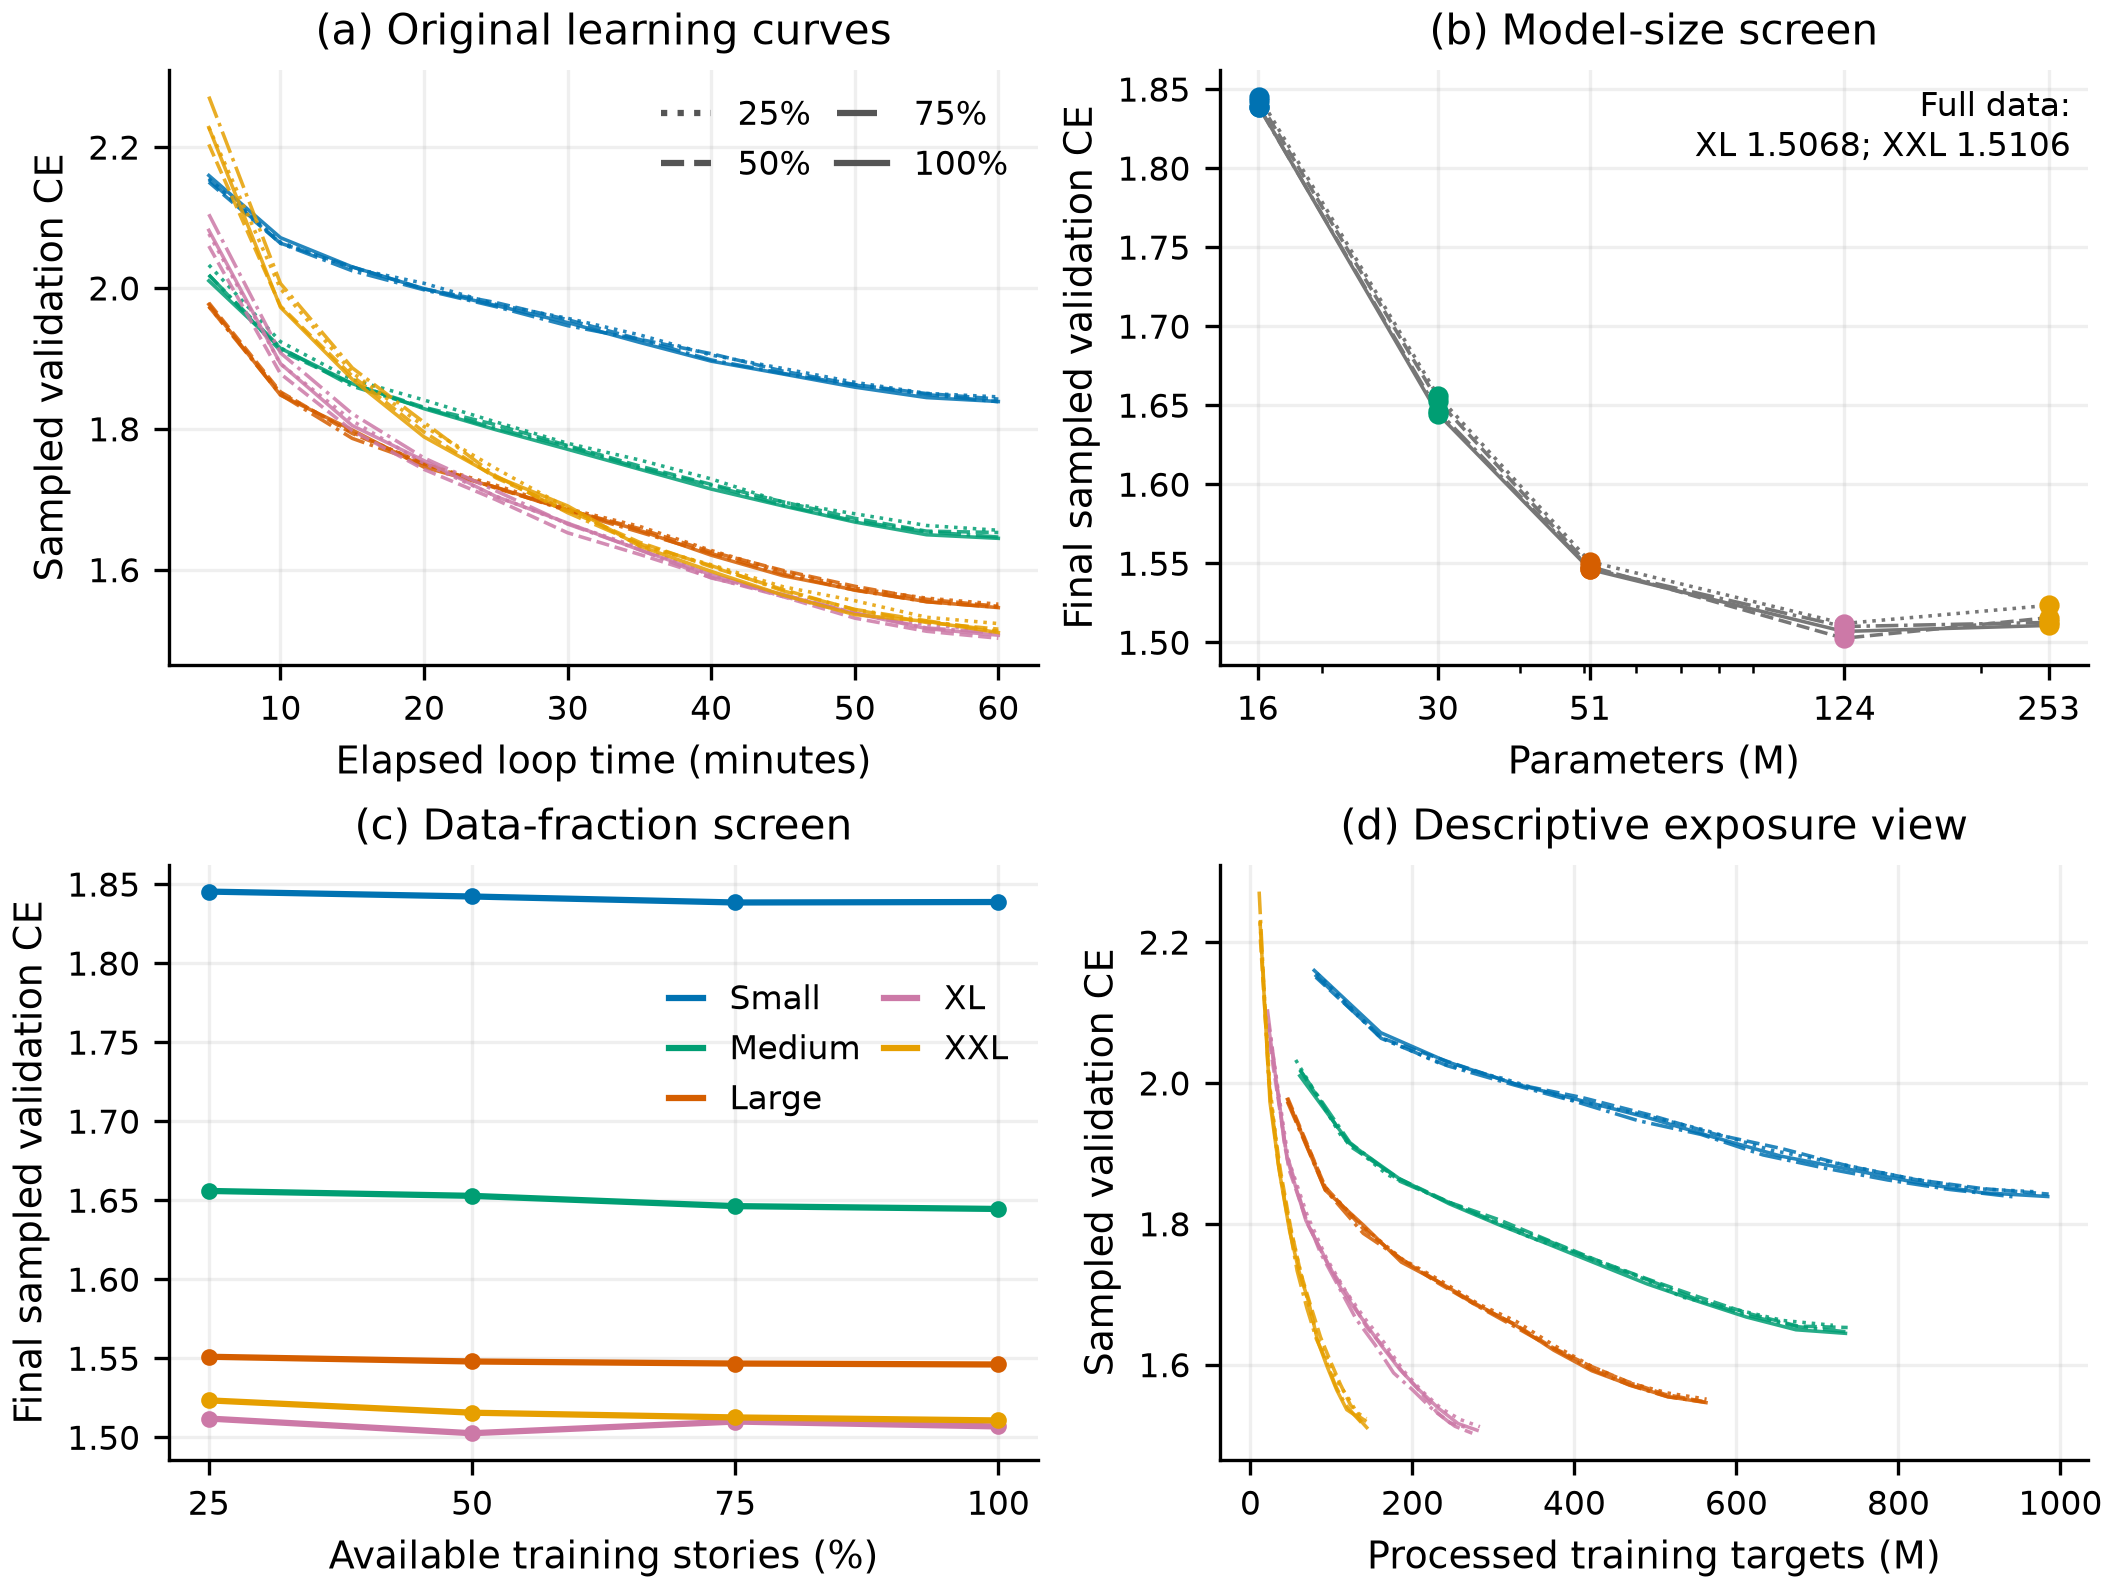
\includegraphics[width=0.74\linewidth]{figures/report2_original_overview.png}
  \caption{The 20-run comparison. (a) Validation CE against time. (b) Final CE
  against model size. (c) Final CE against data fraction. (d) The same curves
  against processed tokens. Colours are sizes, line styles are data fractions.}
  \label{fig:overview}
\end{figure}

\subsection{How many tokens each model sees}
The reason for the flat end of panel (b) is in Table~\ref{tab:sizes}. In the same
hour Small processes 984M tokens and XXL only 144M. The throughput falls by a
factor of 6.9 from Small to XXL. In units of the full training set (474M tokens),
Small sees it 2.08 times, Medium 1.55, Large 1.19, XL 0.59 and XXL 0.30 times. XXL
would need about 3 hours and 18 minutes to see the full data once.

This also corrects an explanation from an early draft, that the data fraction
does not matter because no run finishes one pass. That is wrong for most of the
grid: 15 of the 20 runs process more tokens than their training subset has, and
Small with 25\% of the data goes through its subset 8.2 times. Its loss is still
only 0.007 nats worse than Small with all the data. This agrees with Muennighoff
et al.~\cite{muennighoff2023}, and here it holds up to eight repetitions. A note of
care: windows are sampled with replacement, so ``8.2 times'' counts processed
tokens, it does not mean every story was seen eight times. The token counters in
all 262,432 log rows were also checked to equal steps $\times$ 4096.

\subsection{Is XL really better than XXL?}\label{sec:xlxxl}
The gap between XL and XXL in the first comparison is 0.004 nats, with one seed.
There was a second problem, found late. The validation sample during training was
16 microbatches, and the microbatch size depends on the model. So Small, Medium and
Large were scored on 65,536 tokens, XL on 32,768 and XXL on 16,384. A gap of 0.004
measured like this means very little. Two checks follow.

\textbf{Same validation data.} Four saved checkpoints were scored on the complete
validation set (3,808,643 tokens each). Table~\ref{tab:common} shows that the gap
between XL and XXL grows to 0.034 nats, and XL stays ahead. The order of the two
XL runs changes: with the complete set, 100\% of the data is 0.002 better than
50\%, and before it was the opposite. So the original choice of XL with 50\% data
was inside the noise of a small sample.

\begin{table}[htbp]
\centering\small
\caption{Saved checkpoints scored on the complete validation set, compared with
the sampled validation used during training.}
\label{tab:common}
\begin{tabular}{lrrr}
\toprule
Checkpoint & Sampled CE & Complete CE & Complete PPL \\
\midrule
Large, 100\% & 1.5460 & 1.5469 & 4.697 \\
XL, 50\%     & 1.5025 & 1.4911 & 4.442 \\
XL, 100\%    & 1.5068 & 1.4893 & 4.434 \\
XXL, 100\%   & 1.5106 & 1.5236 & 4.589 \\
\bottomrule
\end{tabular}
\end{table}

\textbf{Three seeds.} XL and XXL were trained again on the full data with seeds 42,
43 and 44, using the same recipe and the same GPU label, and the final checkpoints
were scored on the complete validation set (Table~\ref{tab:seeds},
Figure~\ref{fig:seeds}). XL is better in every pair, and every XL run is better
than every XXL run. The mean CE is 1.4947 for XL (standard deviation 0.0038) and
1.5244 for XXL (0.0098). The mean paired gap is 0.030 nats, which is about 2.9\%
in perplexity (4.458 against 4.592).

This should not be oversold. With three pairs, a paired $t$ interval at 95\%
is $[-0.002,\ 0.061]$, so it includes zero, and three points cannot tell whether the
normal assumption is reasonable. What stands is the same direction three times and a
gap about eight times larger than the spread between XL seeds. That is enough to
call XL the better choice for one hour with this recipe. It is not a significance
test.

\begin{table}[htbp]
\centering\small
\caption{Repeated one-hour runs on the full data. CE on the complete validation
set. A positive gap means XL is better.}
\label{tab:seeds}
\begin{tabular}{rrrrrr}
\toprule
Seed & XL CE & XXL CE & Gap (XXL$-$XL) & XL tokens (M) & XXL tokens (M) \\
\midrule
42 & 1.4904 & 1.5298 & 0.0394 & 271.0 & 138.1 \\
43 & 1.4960 & 1.5303 & 0.0343 & 267.9 & 133.3 \\
44 & 1.4976 & 1.5131 & 0.0155 & 267.9 & 146.4 \\
\bottomrule
\end{tabular}
\end{table}

\begin{figure}[tbp]
  \centering
  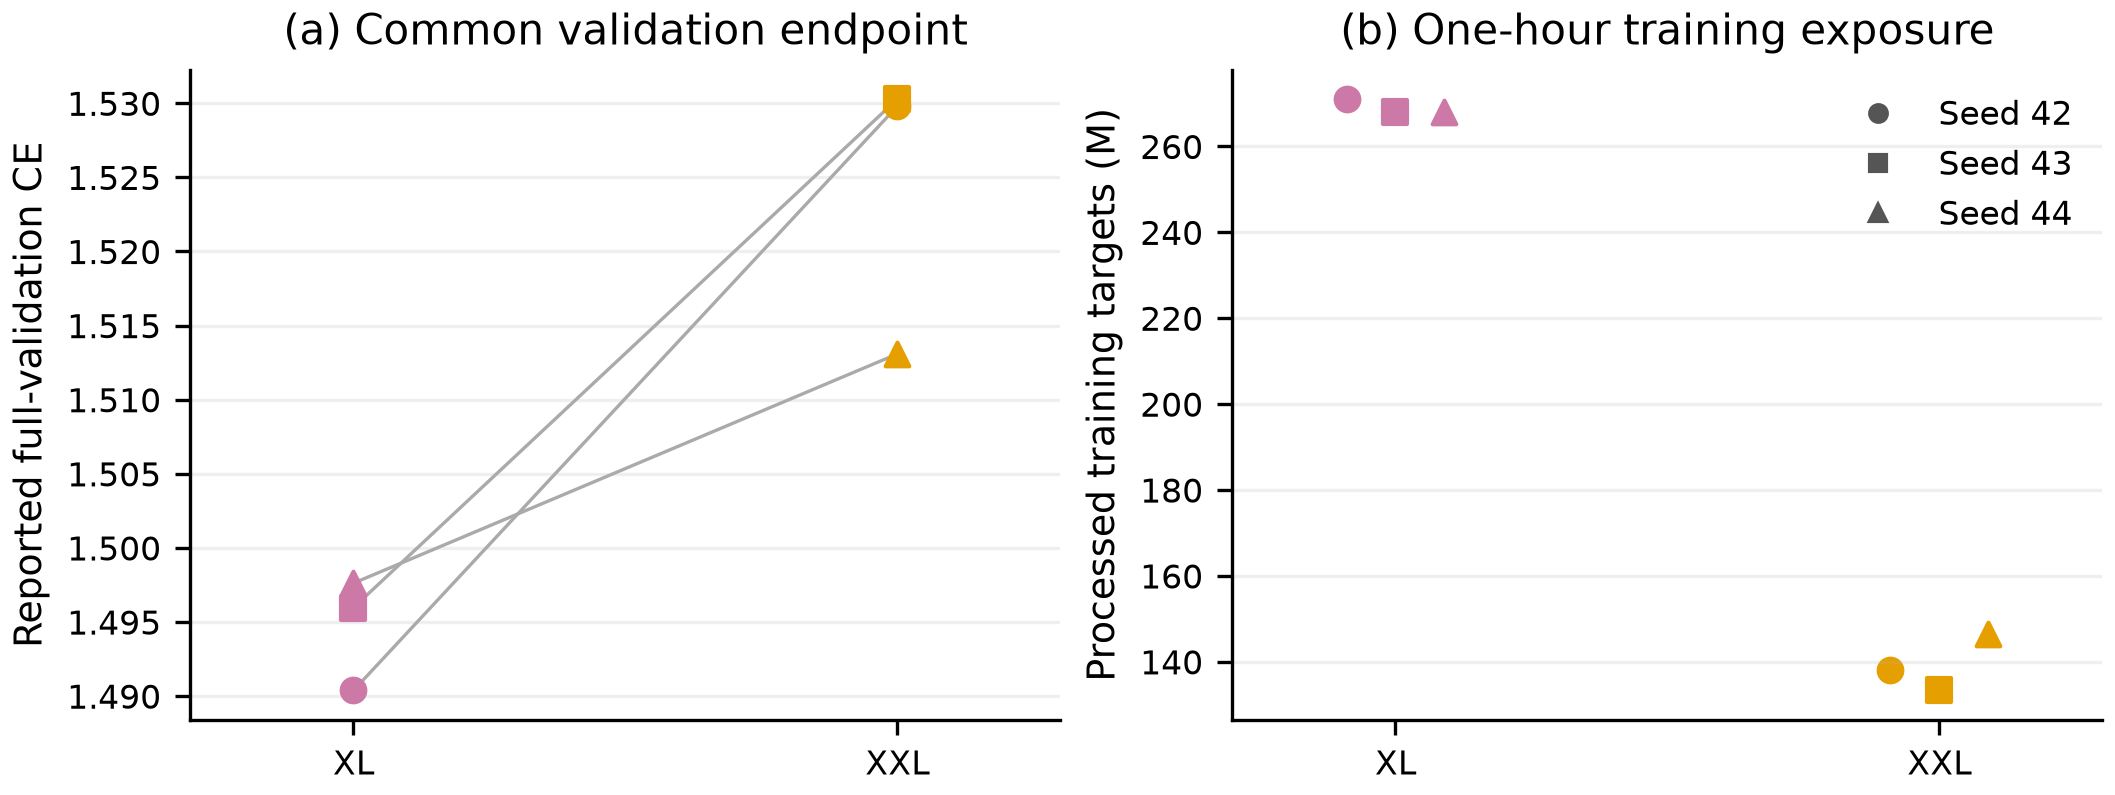
\includegraphics[width=0.68\linewidth]{figures/report2_seed_comparison.png}\\[2pt]
  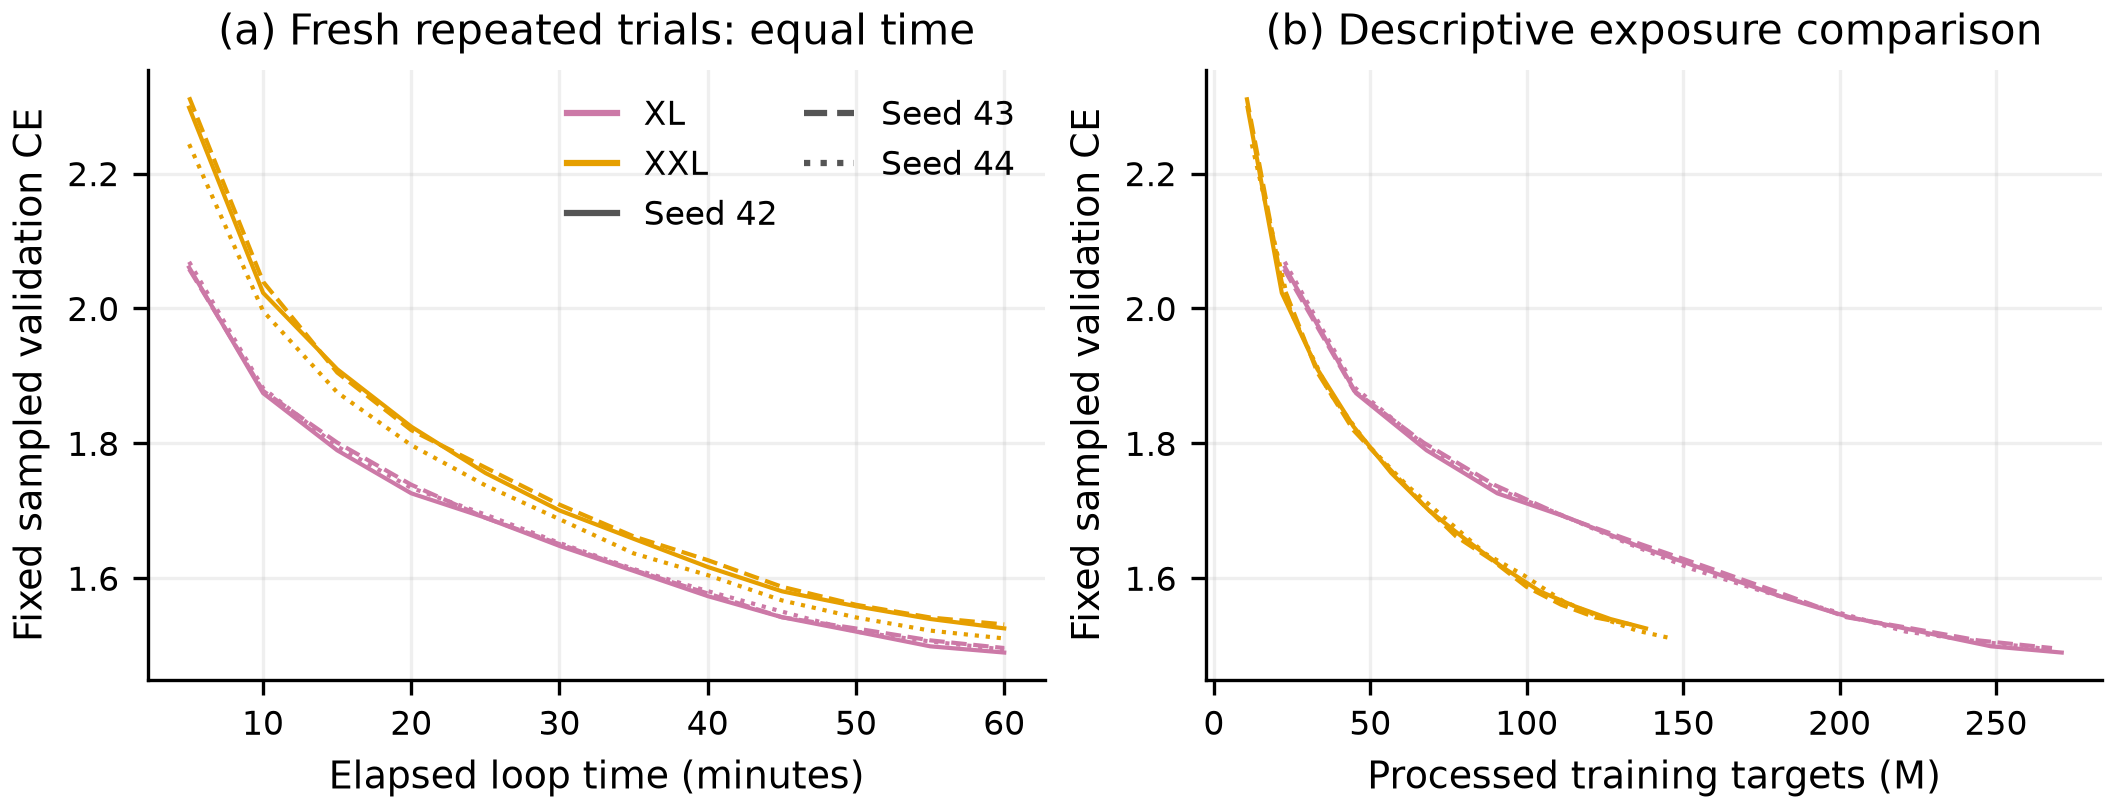
\includegraphics[width=0.68\linewidth]{figures/report2_learning_curves.png}
  \caption{Repeated runs. Top: final CE on the complete validation set and
  processed tokens, by seed. Bottom: sampled validation CE against time (left) and
  against processed tokens (right).}
  \label{fig:seeds}
\end{figure}

One detail in Table~\ref{tab:seeds} is useful. The seed-44 XXL run processed 9.8\%
more tokens than the seed-43 run, on the same GPU label, and it is also the best
XXL run. So the spread between XXL runs is not only the random seed. It is also
how fast the shared GPU was during that hour. For a slow model this matters more.

\textbf{Why XXL loses.} The bottom-right panel of Figure~\ref{fig:seeds} gives the
most interesting reading. At the same number of processed tokens, XXL is ahead: at
120M tokens its CE is about 1.55 and XL is at about 1.68. XXL learns more from
each token, as expected for a larger model. It loses because XL gets 1.93 times as
many tokens in the hour. All six curves are still falling in the last five
minutes, so no model has converged. This suggests XXL is limited by time and not by
capacity. One reading of the curves is confounded, though: the schedule follows the
clock, so at 120M tokens XL is still at a high learning rate and XXL is near the end
of its decay, and part of the gap in that panel can come from this.

\textbf{Matched-token control.} To remove this confound, XL and XXL were trained
from fresh weights for the same 35,000 updates (143,360,000 tokens each), with a
step-based cosine schedule, the same peak learning rate, seed 42 and the same MIG
slice. At equal tokens the ranking flips: XXL reaches complete-validation CE 1.521
against 1.574 for XL, a gap of 0.053 nats (5.2\% in perplexity) in XXL's favour.
XXL needed 62 minutes for these tokens and XL only 31. So, with the clock confound
removed, the extra capacity of XXL does help per token, and it loses in one hour
only because it processes 1.93 times fewer tokens. This is one seeded pair, so the
direction carries more weight than the exact size of the gap.

\subsection{Shorter budget and longer context (exploratory)}\label{sec:extensions}
Four more runs used seed 42 and the full data. With a 30-minute budget, Large has
the lowest validation CE (1.580), then XL (1.633) and XXL (1.680). With one hour XL
is first. So the best size moves up when the budget grows, which is what the token
argument predicts. In the fourth run, XL with context 512 reaches 1.456 against
1.507 for context 256, and it processes fewer tokens (190M against 280M).

These are leads, not results. The four runs were recorded on a GPU labelled
\texttt{H100 NVL}, without the MIG slice, and the throughput is not consistent with
the main runs (Large was faster than before, XL slower). The context-512 run also
doubles the tokens per update, from 4096 to 8192. With these differences it is
unclear how much of each change comes from the budget or from the context.

\subsection{Test results and generated stories}\label{sec:test}
The model selected on validation in the first comparison is XL with 50\% of the
data. Its test CE is 1.4846, the perplexity is 4.41 and it has 0.524 bits per
byte. The test results of all 20 runs are in Table~\ref{tab:all}, and the order of
the sizes is the same as on validation: Small 6.26, Medium 5.16, Large 4.66, XL
4.40 and XXL 4.56 in perplexity for the full-data runs. One caveat: all 20
checkpoints were scored on the test set at the same time, so the test set was seen
before the follow-up decisions. For this reason the repeated runs are compared on
validation only, with no test scores.

Five stories per model were also generated with fixed prompts (temperature 0.8,
top-$k$ 40, 150 new tokens). All models write fluent text in the TinyStories
style, and all of them make errors that the loss does not show. For the prompt
``Tom had a big red ball.'', Small changes the name to Tim, XL has a girl who says
to Tom ``I want to pet you'', and in the XXL story Sam says ``I'm Sam. I'm Tom.''
Five prompts with one sample each cannot rank the models, so no claim follows that
the lower loss of XL gives better stories.

\section{Discussion and limitations}\label{sec:discussion}
The first comparison, the scoring on the complete validation set and the repeated
runs agree: for one hour on this GPU slice with this recipe, the 124M model is the
best of the five. The main trade-off is throughput against capacity. A bigger
model uses each token better but gets fewer of them, and at one hour the balance
is near 124M parameters. The matched-token control makes this explicit: at equal
tokens the larger model is ahead, so the one-hour result is about time, not a
ceiling on what XXL can learn. The 30-minute runs point the same way, with the
balance at a smaller model.

Compared with the literature, the best model here is far from the rule of
Hoffmann et al.: XL sees 280M tokens for 124M parameters, about 2.3 tokens per
parameter and not 20. Large (11 tokens per parameter) and Medium (24) are closer
to the rule and they are clearly worse. The result looks more like the picture of
Kaplan et al., a big model stopped early, up to the point where the model is so
slow that it sees less than a third of the data (XXL). Why the ratio is so low is
unclear. TinyStories is simple and repetitive, and 39M of the XL parameters are the
embedding table, so both things can play a role. The laptop
experiment~\cite{goedecke} was close to the rule with a five-minute budget, so the
ratio may also depend on the budget. One more choice may hurt the large models:
training uses dropout 0.1, while Geiping and Goldstein~\cite{geiping2023} turn
dropout off in their budget setting because it reduces the number of effective
updates. XL and XXL see less than one pass of the data, so dropout is probably not
needed for them, though this was not tested.

The limits are these. First, one learning rate was used for all sizes. Wortsman
et al.~\cite{wortsman2024} show that the loss becomes more sensitive to the
learning rate when the model grows, so XXL was also trained for one hour at half
the peak rate ($1.5\times10^{-4}$); it did not help, with complete-validation CE
rising to 1.546 from 1.530 at the default. One value is not a search, so XXL may
still be at a disadvantage that is not about time. Second, three seeds are few, and
the finalists were chosen after the first results were seen. Third, wall-clock time
is measured on a shared GPU slice, and the speed changed by up to 10\% between runs
of the same model. Fourth, the data fraction results have one seed and differences
of 0.01 nats, so the effect can only be called small. Fifth, the sampled validation
during training used fewer tokens for the bigger models. This surfaced only after
the first comparison, and it is why the checkpoints were scored again.

About reproducibility: configurations, logs and score tables for all runs are in
the repository. All 26 checkpoints (the 20 original runs and the 6 repeated runs)
are in the Hugging Face repository \texttt{dsa4212-tinystories/tinystories-nanogpt},
together with the protocol files of the offline scorer, the per-story scores and
the paired comparisons (\texttt{analysis/followups/}). The offline scoring uses
\texttt{float32}, non-overlapping 256-token windows with the context reset in each
window, and it ran on a GPU labelled \texttt{H100 NVL}. The scoring was not rerun
from the uploaded checkpoints for this report.

The natural next experiments build on the matched-token control: repeating it over
several seeds, and giving XXL a proper per-size learning-rate search rather than the
single reduced rate tried here. A longer wall-clock budget would then show whether
XXL overtakes XL on the clock, which the token accounting predicts but does not
prove.

\section{Conclusion}
With one hour per run, the best model is not the biggest one. XL (124M) beats XXL
(253M) by about 0.03 nats in three repeated pairs, because it processes almost
twice as many tokens. A matched-token control confirms the mechanism: given the same
143M tokens, XXL is ahead by 0.053 nats, so the one-hour ranking is set by
throughput, not capacity. The amount of training data changes little, even when the
small models repeat a quarter of the data eight times. The selected model has a test
perplexity of 4.41. What stays open is whether a longer budget or a per-size
learning rate lets XXL win on the clock, and whether context 512 is really better:
halving XXL's rate for one hour did not help, and the context result is from a single
run on a different GPU label.

{\small
\bibliographystyle{plainnat}
\bibliography{final_references}
}

\appendix
\section{All 20 runs and how to reproduce them}
The commands are in \texttt{README.md}: \texttt{run.py prepare}, \texttt{run.py
train} and \texttt{run.py evaluate}, each with a file from \texttt{configs/}.
\texttt{eval\_hf.py} scores the saved checkpoints on the test set and
\texttt{analyze.py} builds the tables and figures. Per-run logs are in
\texttt{results/} and \texttt{runs/}; the follow-up configs are in
\texttt{configs/followups/} and the score tables of Section~\ref{sec:xlxxl} are in
\texttt{analysis/followups/} (seed, matched-token and learning-rate subfolders).

\begin{table}[h!]
\centering\scriptsize\renewcommand{\arraystretch}{0.85}
\caption{The 20-run comparison (seed 42, one hour). ``Passes'' is processed tokens
divided by the size of the training subset. Validation is the sampled one, test is
the full test set (957,184 tokens).}
\label{tab:all}
\begin{tabular}{lrrrrrrr}
\toprule
Size & Data (\%) & Tokens (M) & Passes & Val CE & Test CE & Test PPL & Test bpb \\
\midrule
Small  &  25 & 972.0 & 8.21 & 1.8452 & 1.8422 & 6.311 & 0.650 \\
Small  &  50 & 985.5 & 4.16 & 1.8421 & 1.8396 & 6.294 & 0.649 \\
Small  &  75 & 940.8 & 2.65 & 1.8383 & 1.8378 & 6.283 & 0.648 \\
Small  & 100 & 984.3 & 2.08 & 1.8386 & 1.8340 & 6.259 & 0.647 \\
Medium &  25 & 719.1 & 6.07 & 1.6558 & 1.6502 & 5.208 & 0.582 \\
Medium &  50 & 737.3 & 3.11 & 1.6527 & 1.6485 & 5.199 & 0.582 \\
Medium &  75 & 738.3 & 2.08 & 1.6462 & 1.6430 & 5.171 & 0.580 \\
Medium & 100 & 734.6 & 1.55 & 1.6444 & 1.6415 & 5.163 & 0.579 \\
Large  &  25 & 563.2 & 4.75 & 1.5509 & 1.5475 & 4.700 & 0.546 \\
Large  &  50 & 557.9 & 2.35 & 1.5479 & 1.5445 & 4.686 & 0.545 \\
Large  &  75 & 562.0 & 1.58 & 1.5466 & 1.5408 & 4.668 & 0.544 \\
Large  & 100 & 562.4 & 1.19 & 1.5460 & 1.5390 & 4.660 & 0.543 \\
XL     &  25 & 283.3 & 2.39 & 1.5118 & 1.4918 & 4.445 & 0.526 \\
XL     &  50 & 273.9 & 1.16 & 1.5025 & 1.4846 & 4.413 & 0.524 \\
XL     &  75 & 269.1 & 0.76 & 1.5099 & 1.4890 & 4.433 & 0.525 \\
XL     & 100 & 279.8 & 0.59 & 1.5068 & 1.4824 & 4.403 & 0.523 \\
XXL    &  25 & 143.2 & 1.21 & 1.5233 & 1.5291 & 4.614 & 0.539 \\
XXL    &  50 & 148.2 & 0.63 & 1.5155 & 1.5182 & 4.564 & 0.536 \\
XXL    &  75 & 141.1 & 0.40 & 1.5125 & 1.5231 & 4.587 & 0.537 \\
XXL    & 100 & 143.7 & 0.30 & 1.5106 & 1.5174 & 4.560 & 0.535 \\
\bottomrule
\end{tabular}
\end{table}

\end{document}
